\newgeometry{margin=2cm}
\section{Anhang: Beispielhafte Klone}

\begin{figure}[h!]
  \centering
  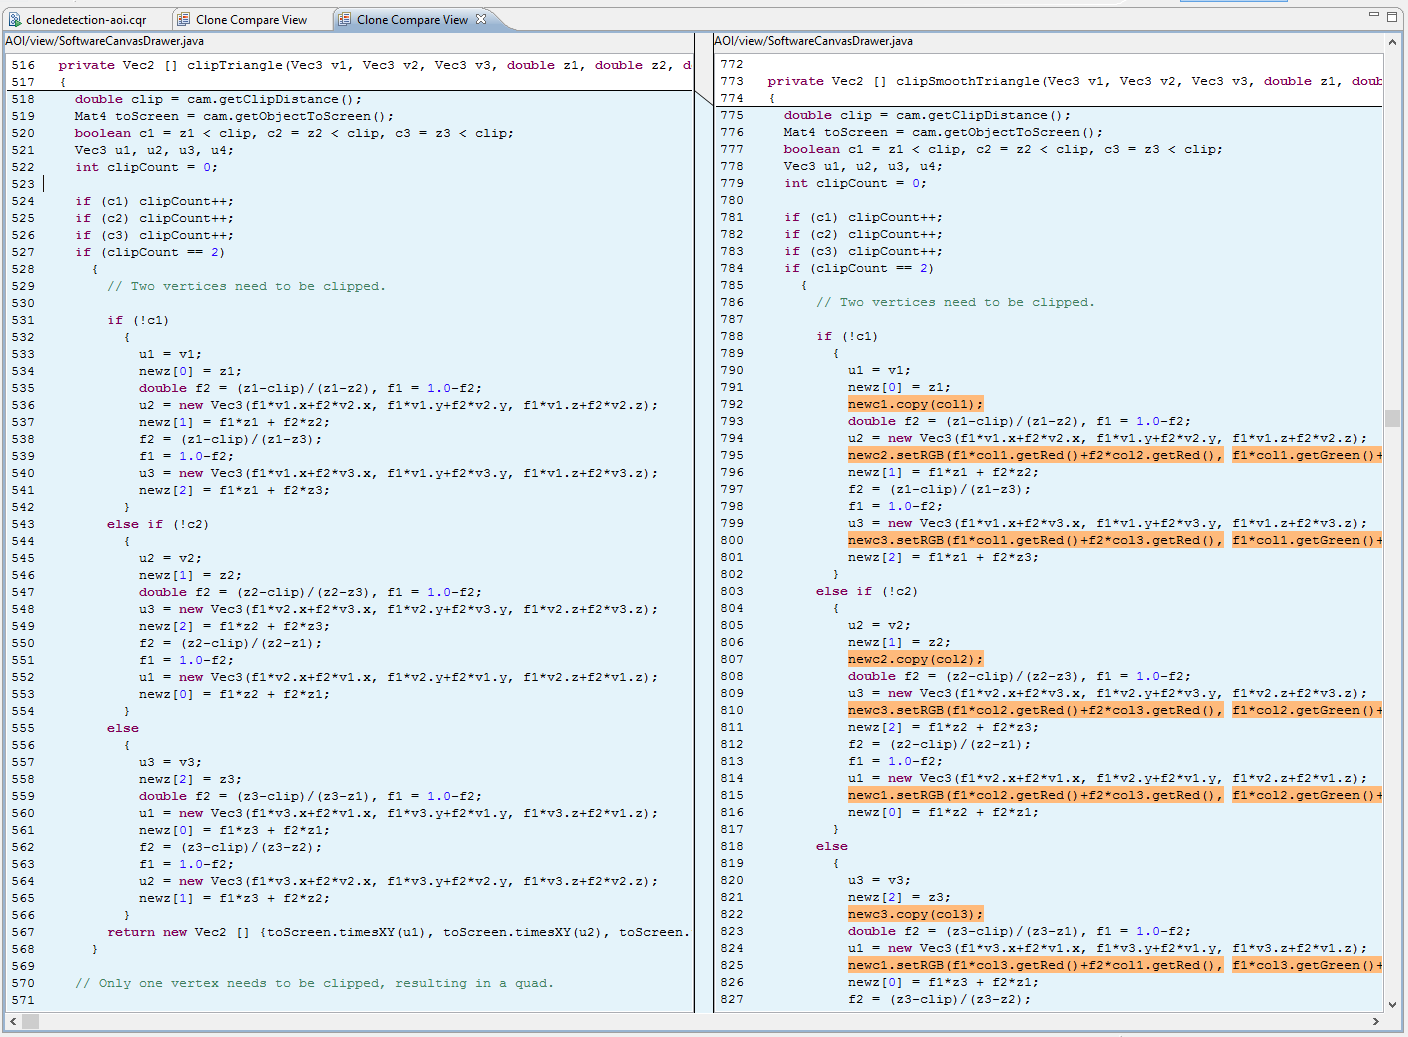
\includegraphics[width=\textwidth]{imgs/clone_examples/gapped_clip_triangle.PNG}
  \caption{Beginn eines langen Klons in AoI}
\end{figure}


\begin{figure}[h!]
  \centering
  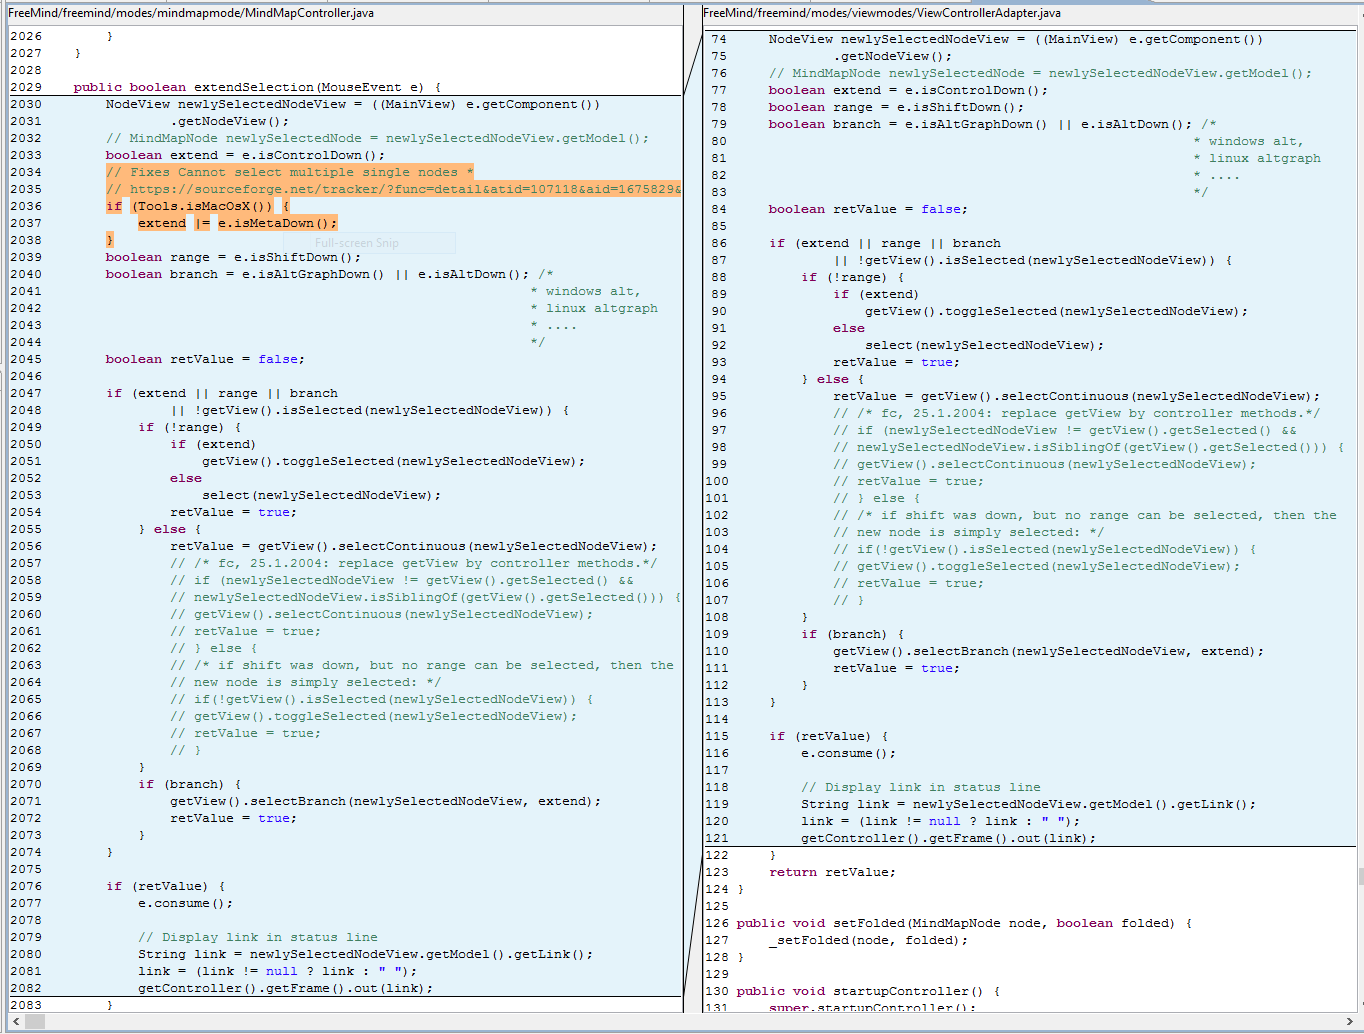
\includegraphics[width=\textwidth]{imgs/clone_examples/freemind_fix.PNG}
  \caption{Möglicherweise unabsichtlich inkonsistenter Bugfix in FreeMind (\#1)}
\end{figure}


\begin{figure}[h!]
  \centering
  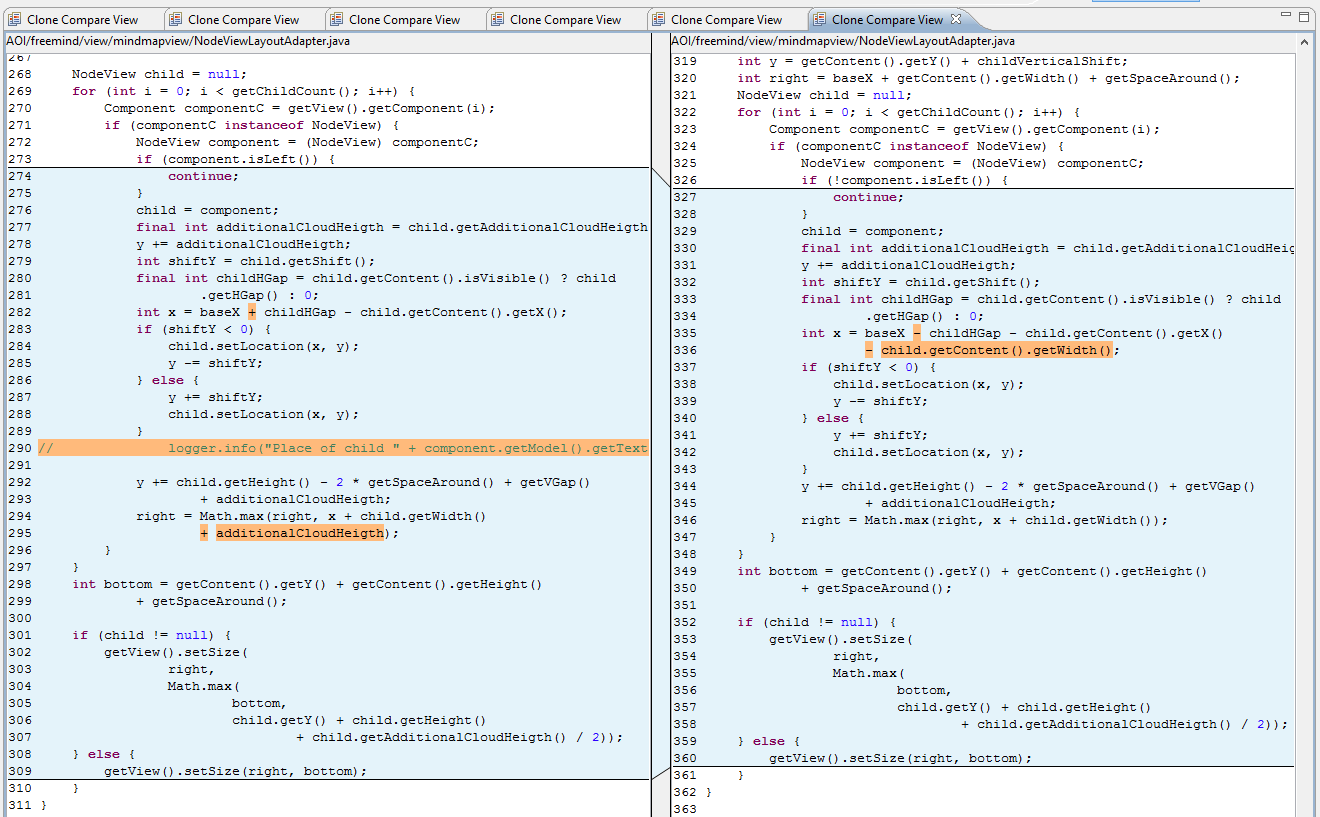
\includegraphics[width=\textwidth]{imgs/clone_examples/additional_cloud_height_bug.PNG}
  \caption{Möglicherweise unabsichtlich inkonsistenter Bugfix in FreeMind (\#2)}
\end{figure}


\begin{figure}[h!]
  \centering
  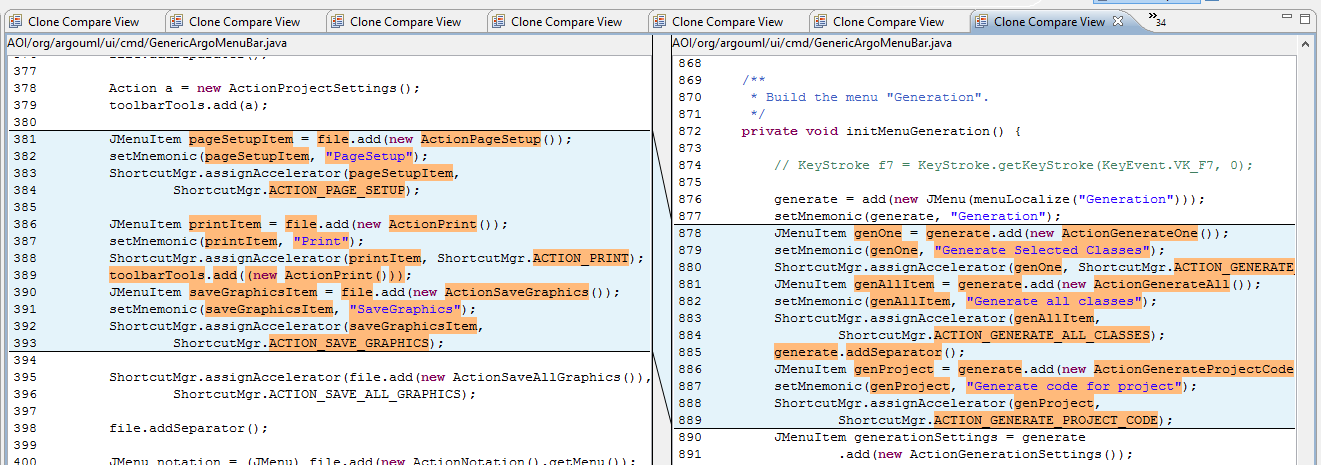
\includegraphics[width=\textwidth]{imgs/clone_examples/false_positive_ui_boilerplate.PNG}
  \caption{Ein \textit{false positive} in Argo\textsc{Uml}}
\end{figure}


\begin{figure}[h!]
  \centering
  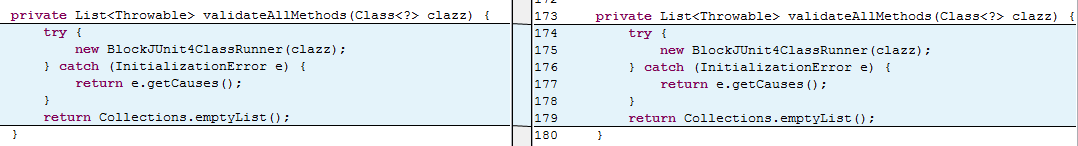
\includegraphics[width=\textwidth]{imgs/clone_examples/junit_uninteresting.PNG}
  \caption{Ein uninteressanter Klon ohne Gaps in JUnit}
\end{figure}


